\section{Fundamentals}

To understand how \lare{} works a few technologies are required to know about.
\html{}, the markup language which is used to create \webPage{}s, is the first technology which is required to know about.
Afterwards \httpRequest{}s are declared as the fundamental transfer protocol of the World Wide Web.
Dynamic content and synchronicity are the topics explained next, which is the problem which is addressed by \ajax{} and \singlePageApplication{}s, which are presented subsequently.
The History API released in October 2014 and required by \lare{} is presented at the end of this chapter.

\subsection{\html{}\label{html}}
Hypertext Markup Language is the language which is used to create webpages.
It allows to structure a web document semantically, but not to style it.
Similar to XML it consists of hierarchically structured tags.
Each tag may have attributes.
Allowed attributes are defined per tag, e.g. an anchor tag may have an href attribute, which is not allowed on a div tag.
There is a special tag, called ID which defines the unique identifier of a tag.
Each value may not occur more than once on a page.

\subsection{\httpRequest{}\label{httpRequest}}
The world wide web has one main protocol to let web-browsers and web-servers communicate, the Hypertext Transfer Protocol (\http{}), which is built on top of the Transmission Control Protocol (TCP).
TCP and so \httpRequest{}s always start with a handshake to establish a connection before data is transferred.
After this handshake, the client sends the request data to the web-server.
This recognizes and interprets the request and if the requested resource is available, sends the according data back, otherwise it sends an error.
Typically it renders data out of a database into a \html{} template and sends it back as the response.
The browser receives this \webPage{} interprets and renders it.
Subsquently it sends \httpRequest{}s to receive the images, CSS and scripts linked in this page.
\begin{figure}[H]
\centering
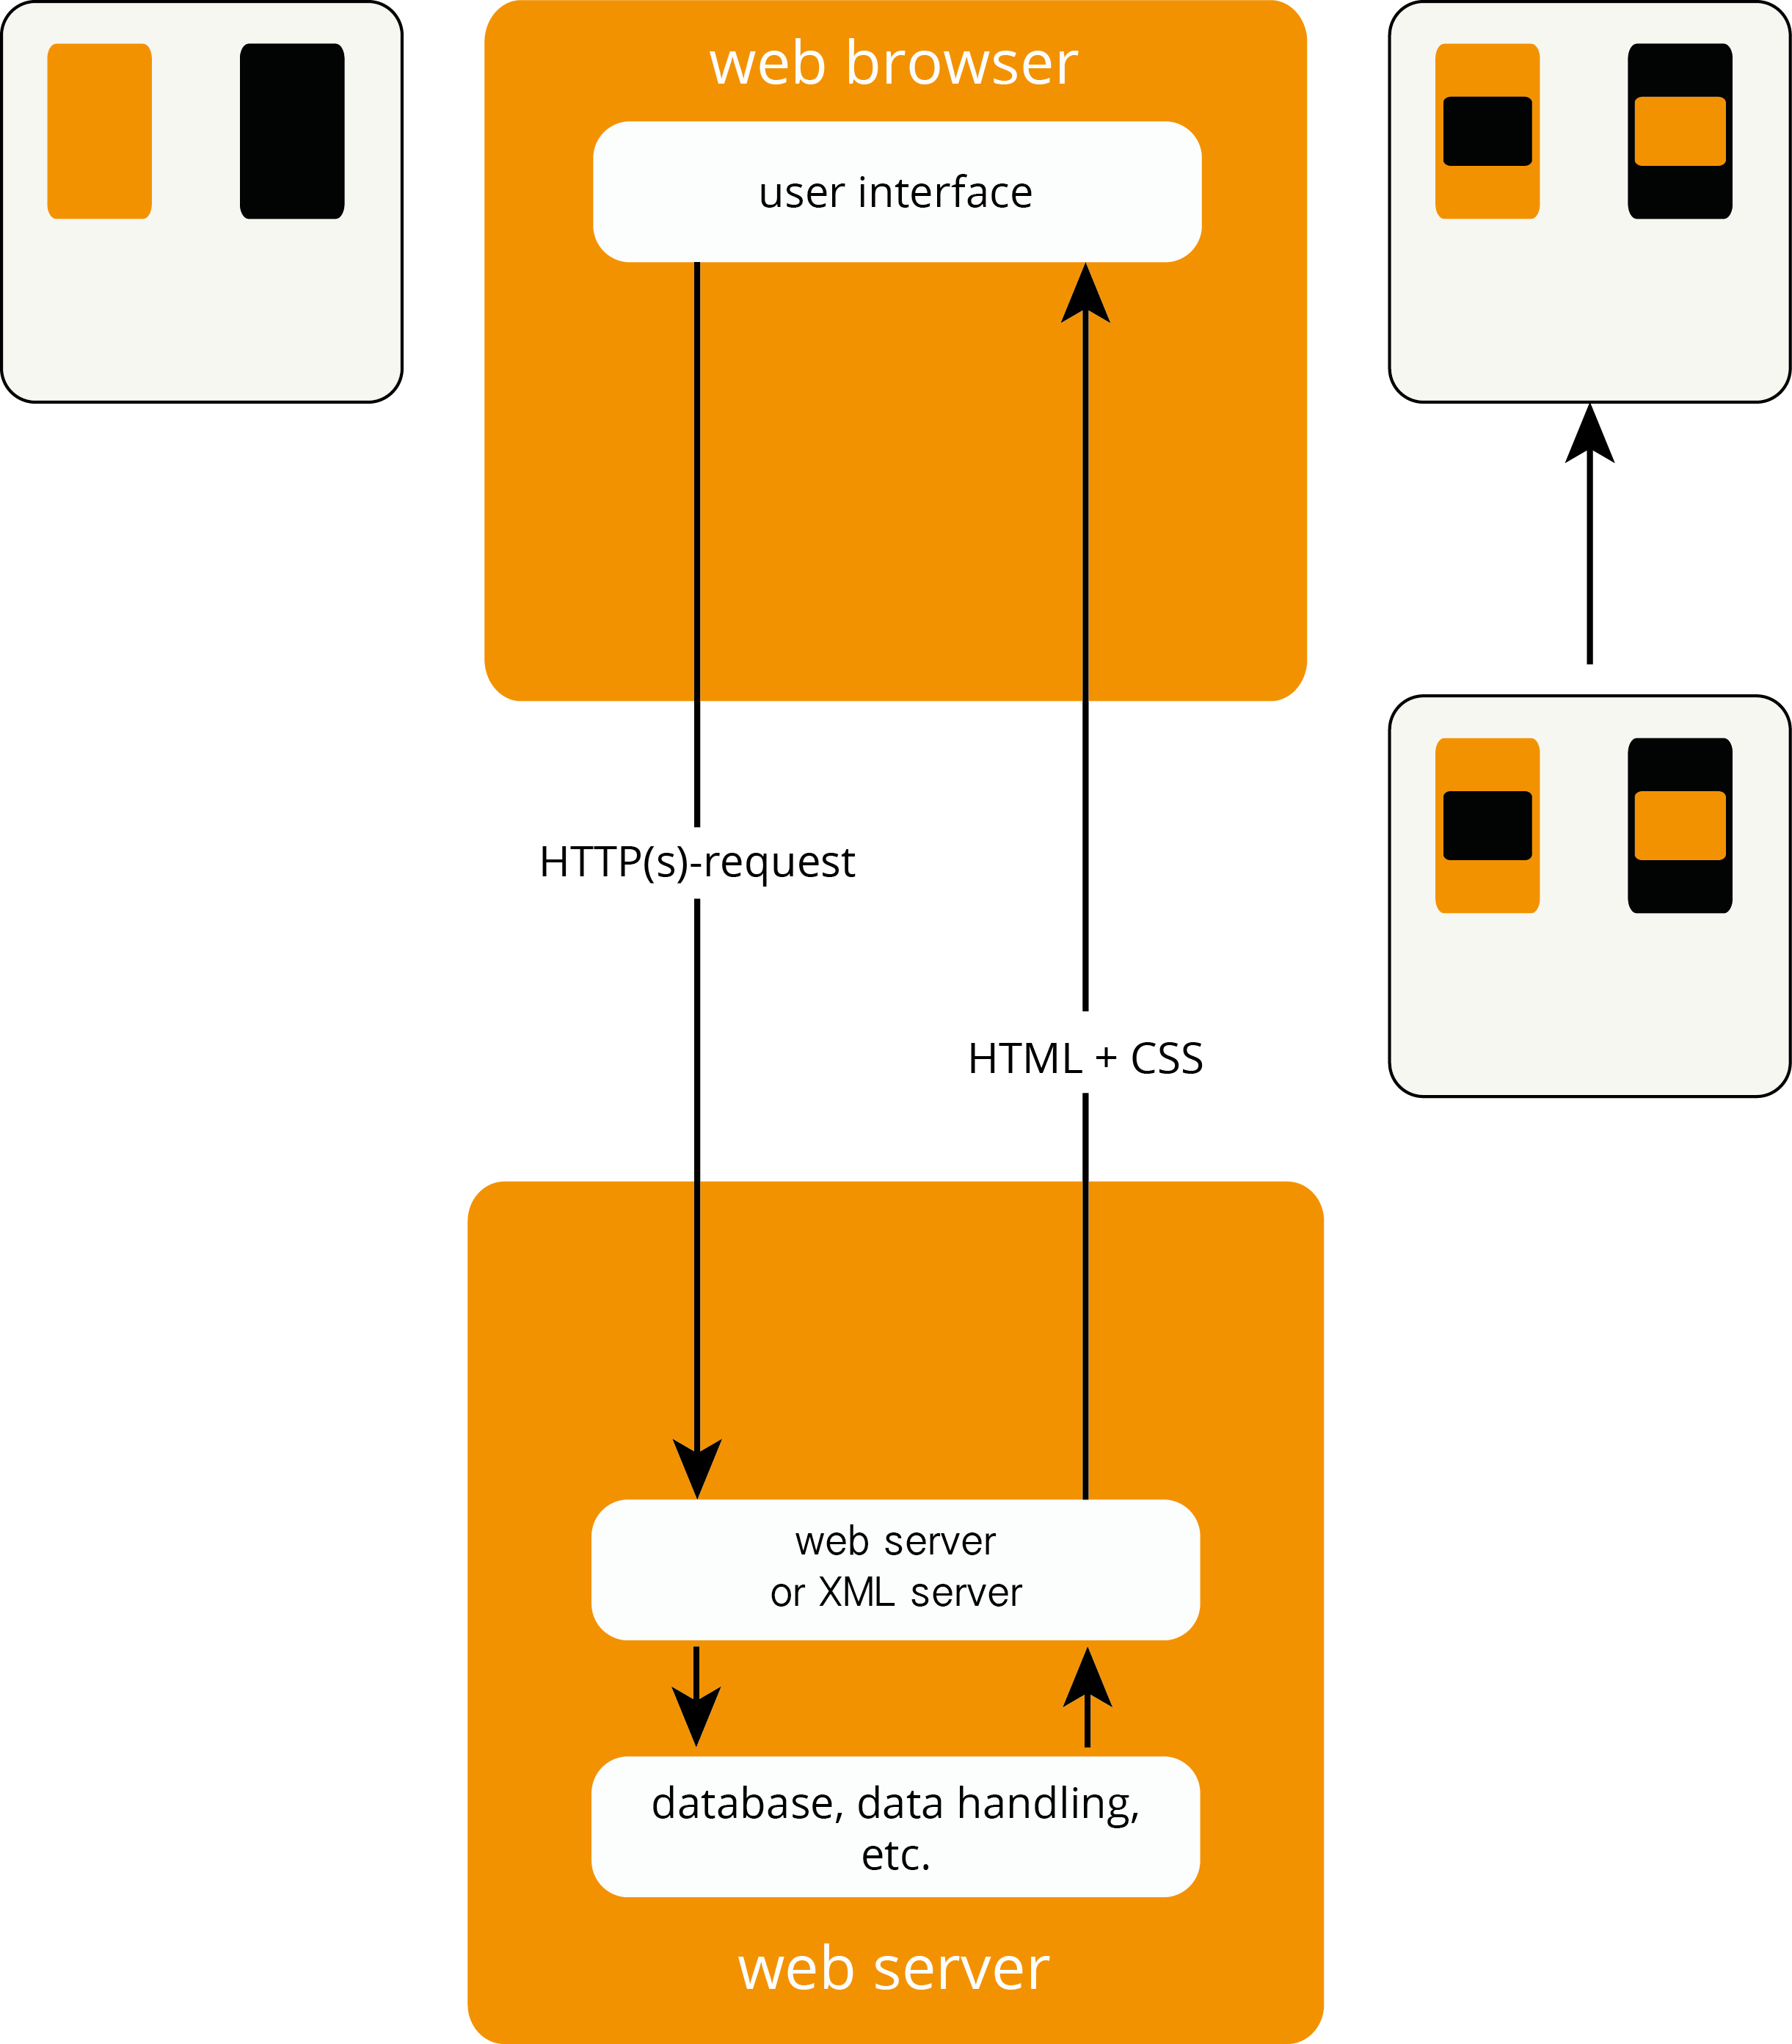
\includegraphics[height=13cm]{images/http.png}
\caption[http_components]{Component and communication diagram of \http{}}
\label{fig:http_components}
\end{figure}

\subsection{Dynamic content and synchronicity\label{synchronicity}}
Dynamic content in websites is content which is changed within an already fully loaded web page, without loading another full page including all resources. 
The normal \httpRequest{}, which is described in \ref{httpRequest}, does not support dynamic changes of content. 
To retrieve new information the client has to request another full web page, including all resources and data which is necessary, which makes this model \enquote{synchronous}.
An \enquote{asynchronous} model is able to change content dynamically without having to load a whole page. 
\ajax{}, as shown in \ref{ajax}, is the most used technique for asynchronous web platforms.

\subsection{\ajax{}\label{ajax}}
Asynchronous JavaScript and XML is a technology to implement dynamic \webPage{}s.
JavaScript is used to make requests to a web server without loading a full new page.
The response then is interpreted by an \ajax{}-engine.
\begin{figure}[H]
\centering
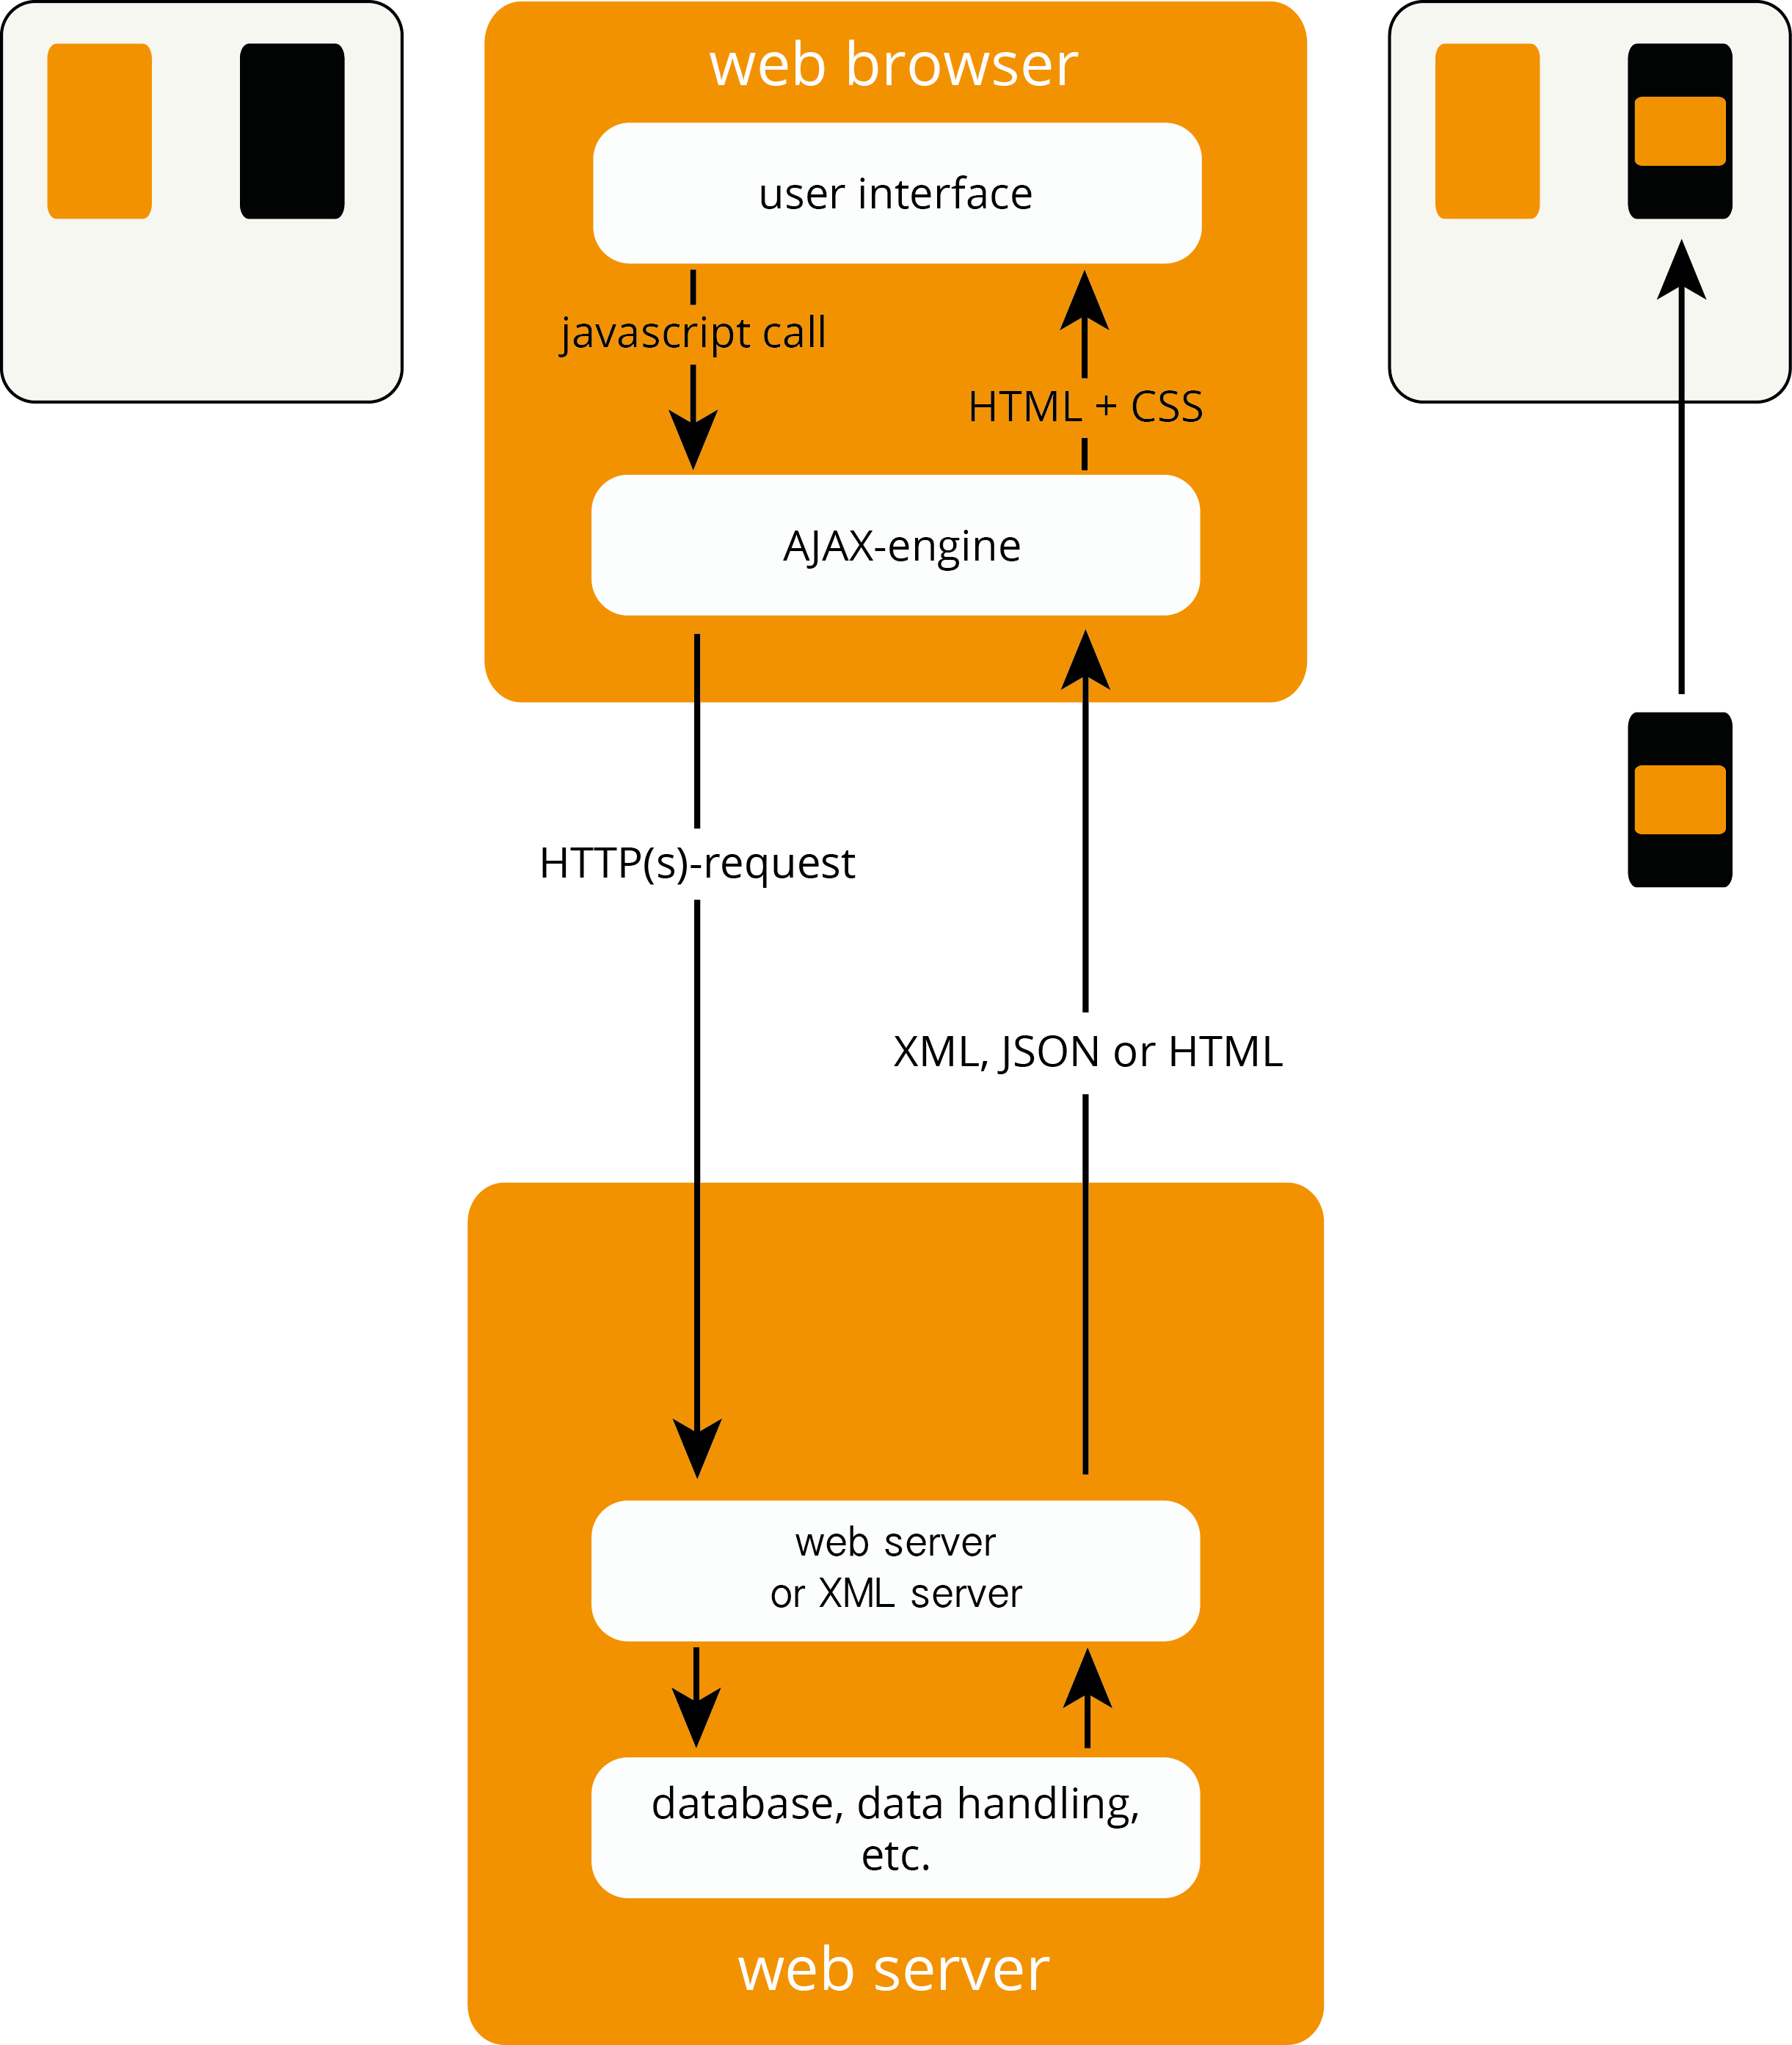
\includegraphics[height=13cm]{images/ajax.png}
\caption[ajax_components]{Component and communication diagram of \ajax{}}
\label{fig:ajax_components}
\end{figure}    
As shown in \ref{fig:http_components} a normal \http{} request by a browser forces the requests always to be synchronous, which means that the client has to wait for a fully loaded page on every request.
Through the \enquote{Asynchronous JavaScript and XML}, short \ajax{}, this can be improved.
The data flow in AJAX is very similar to the normal browser behaviour, but is using a new, third layer: the \enquote{\ajax{}-engine}.
The first request to a web-server using \ajax{} is the complete same as one without \ajax{} with the exception, that one of the requested sources is a JavaScript, which instantiates a \ajax{}-engine.
The following requests now are handled by this \ajax{}-engine, allowing to request web-sources asynchronously.
Without using \ajax{} after receiving \html{}, the browser renders the whole page, even if there are only small changes to the page rendered before.
\ajax{} instead only requests small parts of a website, most of the time in XML or JSON format, interprets it and then only adds, replaces or appends old content with the newly received.

\subsection{\SinglePageApplication{}s\label{singlePageApplication}}
A single-page application is a web application or \webSite{} that only needs to one full \webPage{} load.
Beside this there is no \webPage{} loaded completely at any point in the process anymore.
Often content changes are made asynchronous and dynamically by \ajax{} in response to user actions.
A disadvantage of a lot of \singlePageApplication{}s is the lack of browser history support.
When changing the content the browser does not interpret it as a new page, but only changed content.
This leads into a missing functionality of forward- and back-buttons in browsers.

Additionally a problem of SPAs is, that it has a huge impact on SEO.
The \webPage{} is often rendered inside the browser, and not structured into different URLs.
Those facts make it hard for a search-engine to discover it.

\subsection{History API}
The history API is part of HTML5 specification by \gls{w3c}.
It describes the API for interface for an History object which is part of the session history.
This session history enables functionality like the back-and forward-buttons on browsers.
Defined as a list of session history entries, it represents the browsing history.
A session history entry may be a URL or a state object and may have additional information.

We need to influence this list in \lare{} via the History interface.
This is possible via the window.history.pushState(data, title[, url]) method, which allows to add a new state into this list.
